\begin{definition}[Дисперсия]
\[\D\xi = \E (\xi - \E\xi)^2.\]
\end{definition}

\begin{statement}
\[\D\xi = \E\xi^2 - (\E\xi)^2.\]
\end{statement}
\begin{proof}
Из определения и свойства линейности мат. ожидания.
\end{proof}

\begin{definition}(Ковариация)
\[cov(\xi, \eta) = \E(\xi - \E\xi)(\eta - \E\eta).\]
\end{definition}
\begin{statement}
\[\D\xi = cov(\xi, \xi).\]
\end{statement}

\subsubsection*{Свойства}
\begin{itemize}
    \item $\D\xi \geqslant 0$.
    \item $\D(c\eta) = c^2 \D\eta$.
    \item $cov(\xi, \eta) = \E\xi\eta - \E\xi \cdot \E\eta$.
    \begin{proof}
    Расписать ковариацию и воспользоваться линейностью мат. ожидания.
    \end{proof}
    \item $cov(\xi, \eta) = cov(\eta, \xi).$\\
    $cov(a_1\xi_1 + a_2\xi_2, \eta) = a_1 cov(\xi_1, \eta) + a_2 cov(\xi_2, \eta)$.
    \item $D(\xi_1 + \ldots + \xi_n) = \sum_{i=1}^n\D\xi_i + \sum_{i \neq j} cov(\xi_i, \xi_j).$
    \begin{proof}
    \(\D(\xi_1 + \ldots + \xi_n) = cov(\xi_1 + \ldots + \xi_n, \xi_1 + \ldots + \xi_n) = \sum_{i, j} cov(\xi_i, \xi_j).\)
    \end{proof}
    \item Если $\xi \indep \eta$, то $cov(\xi, \eta) = 0$.
    \item Если $\xi_1, \ldots \xi_n$~--- попарно независимы, то\\
    \(\D(\xi_1 + \ldots + \xi_n) = \D\xi_i + \ldots \D\xi_n\).
\end{itemize}
\begin{definition}(Корреляция)
\[\rho(\xi, \eta) = \frac{cov(\xi, \eta)}{\sqrt{\D\xi}\sqrt{\D\eta}}.\]
\end{definition}

Теорема о мат. ожидании произведения для независимых случайных величин доказана как пункт~(\ref{mathexp-trait-independ}) свойств.

\subsubsection*{Примеры}
\noindent 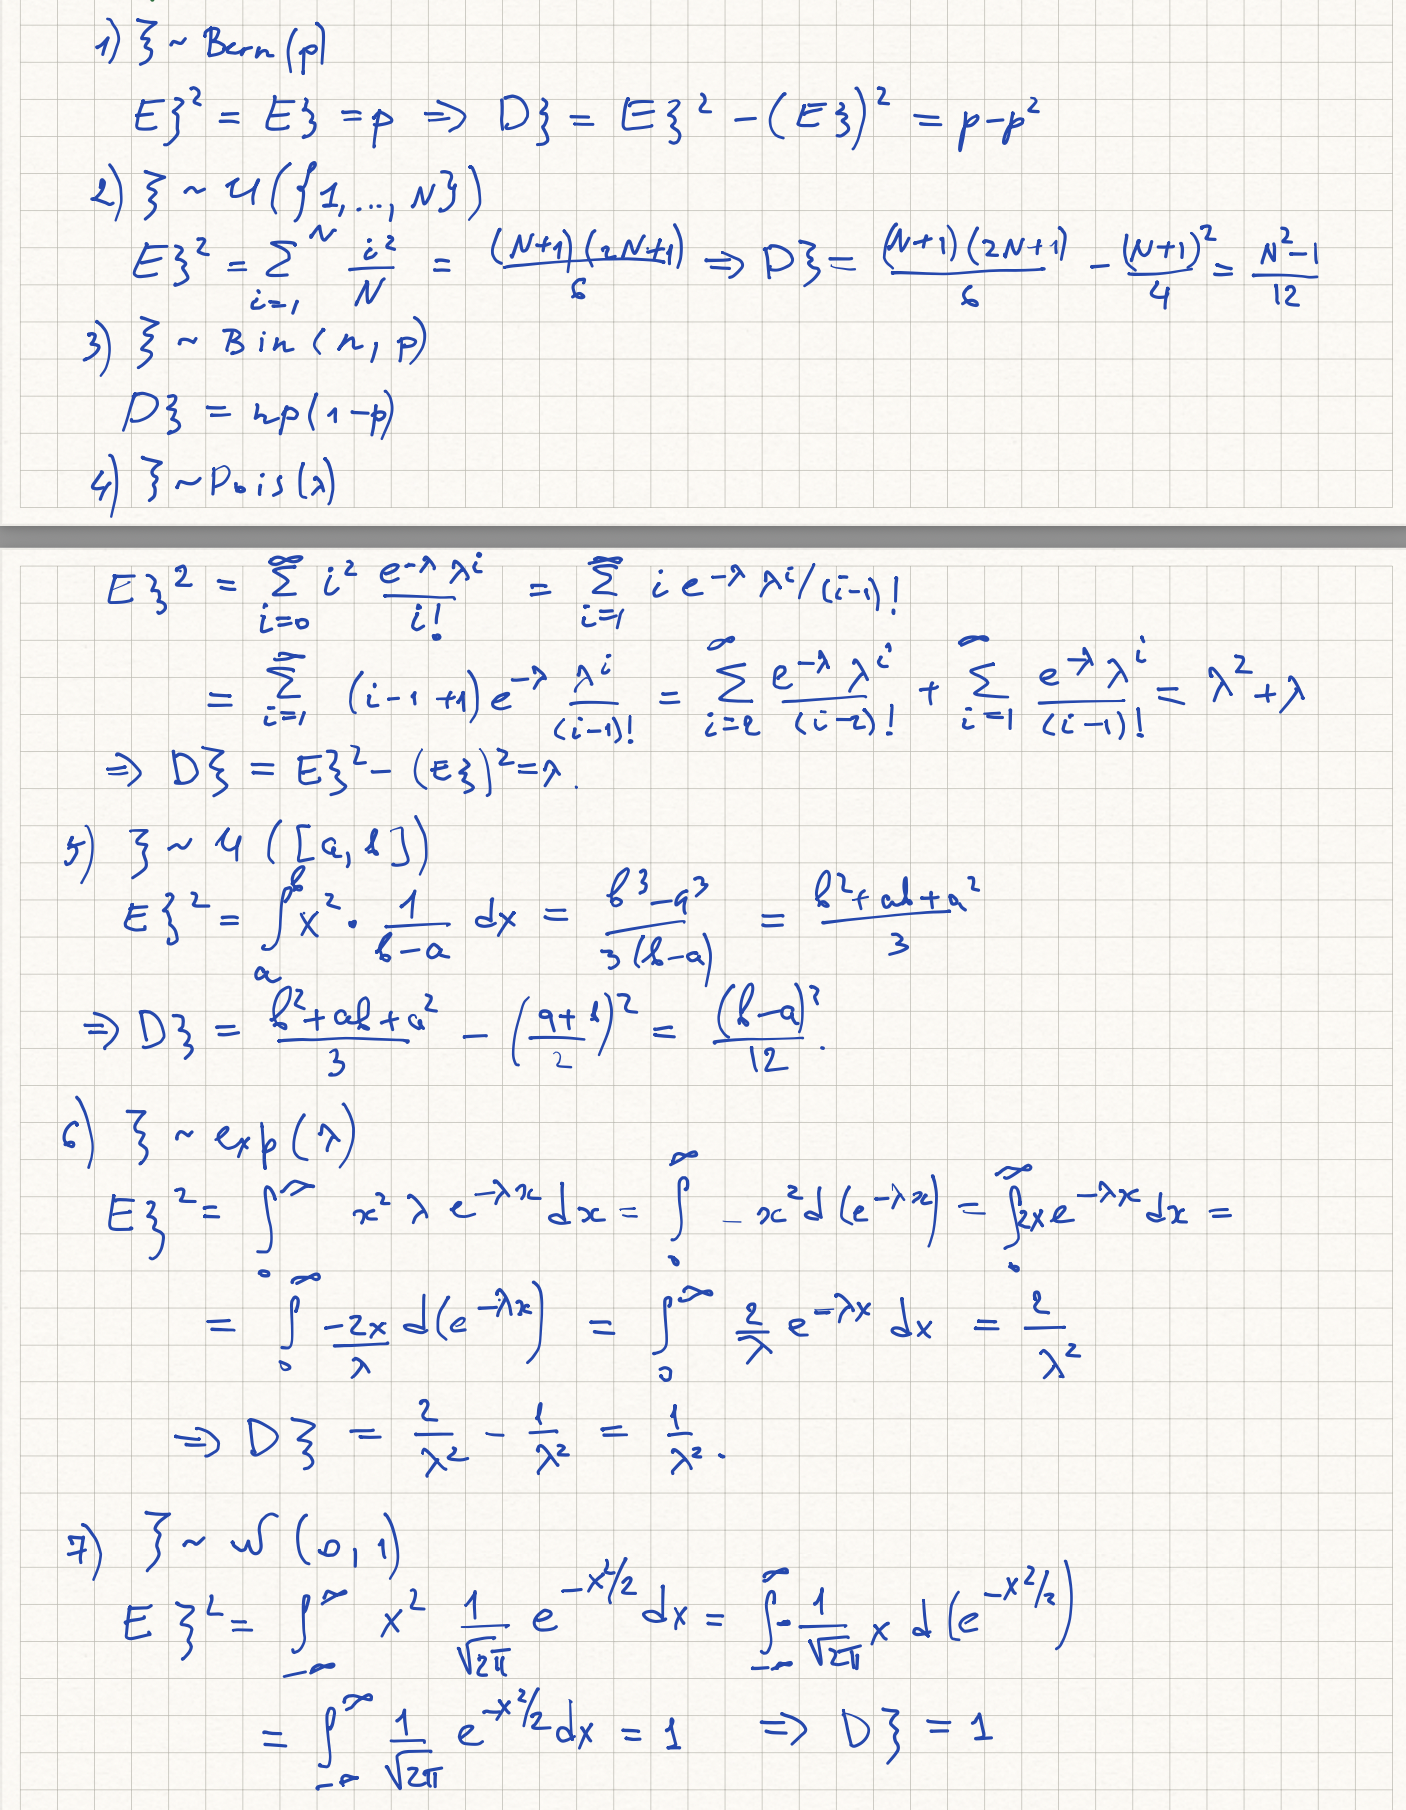
\includegraphics[width=1\linewidth]{sections/sasha/images/expect-example-2.png}
\newpage
\noindent 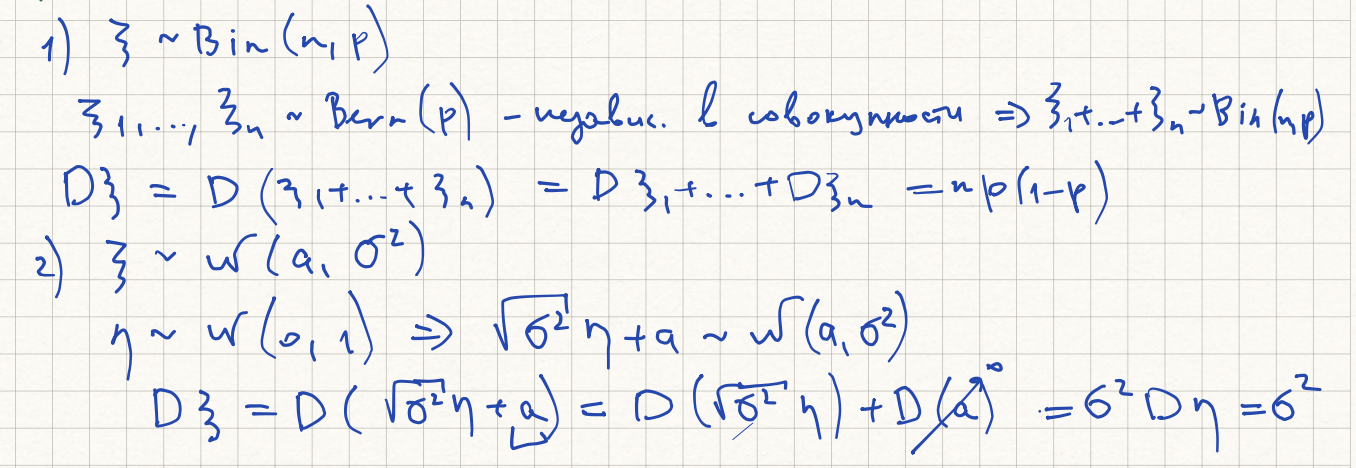
\includegraphics[width=1\linewidth]{sections/sasha/images/expect-disp-ex.png}